%% Figure: compile rate vs behavioral pass rate in the 18 papers that report both
%% for the same outputs (recount 25/10/2026, revised after an independent check;
%% sheet "Mã hoá tổng hợp", column "Nhiều oracle trên cùng output", group "Hình 3";
%% numbers from field 6 of "Trích xuất (nháp)", checked against the papers).
%% Each row: (compile rate, behavioral pass rate) as reported; rows sorted by gap.
%% Fractions used: DepUpgrade 119/123 and 62/123 (equivalent patches over all
%% tasks); Fruntke & Krinke 40/65 and 12/65; VERT 539/569 and 295/569;
%% IntentTester 2,776/3,257 and 1,996/3,257; RISE 136/143 and 124/143;
%% Translation Tag Team 274/350 and 253/350; BatFix 605/698 and 567/698.
%% If a value changes, edit it here AND the gap label on the right.
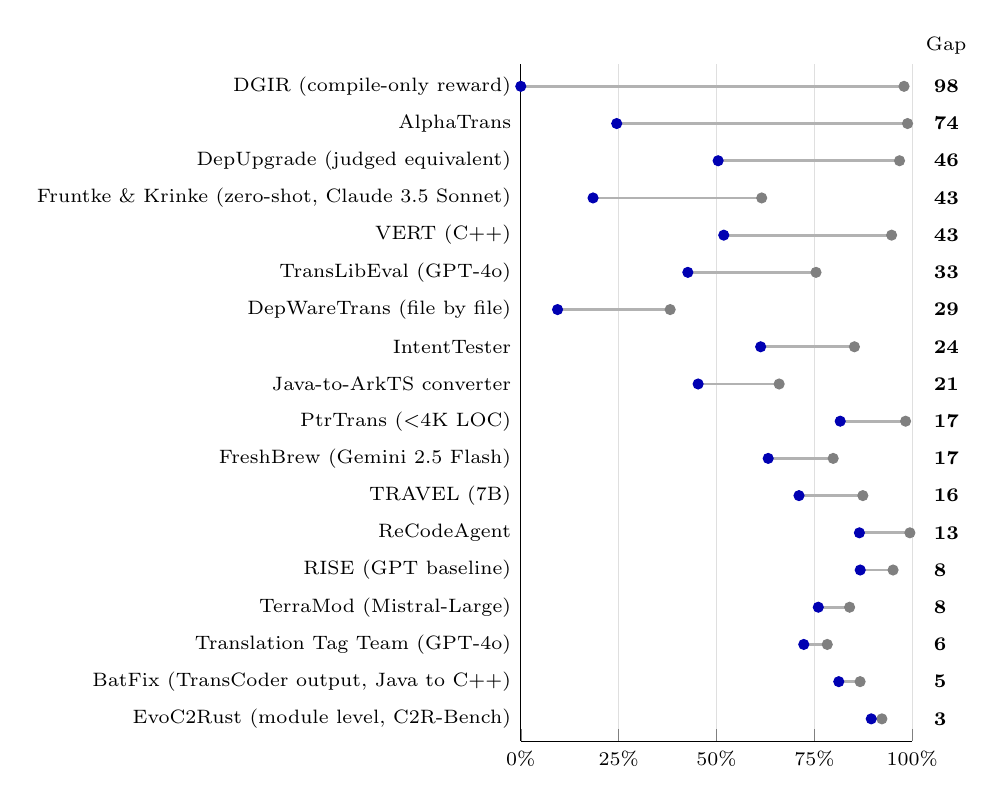
\begin{tikzpicture}
\begin{axis}[
  scale only axis, width=0.41\columnwidth, height=8.6cm,
  xmin=0, xmax=100, ymin=0.4, ymax=18.6, y dir=reverse,
  ytick={1,...,18}, yticklabels={{DGIR (compile-only reward)},{AlphaTrans},{DepUpgrade (judged equivalent)},{Fruntke \& Krinke (zero-shot, Claude 3.5 Sonnet)},{VERT (C++)},{TransLibEval (GPT-4o)},{DepWareTrans (file by file)},{IntentTester},{Java-to-ArkTS converter},{PtrTrans ($<$4K LOC)},{FreshBrew (Gemini 2.5 Flash)},{TRAVEL (7B)},{ReCodeAgent},{RISE (GPT baseline)},{TerraMod (Mistral-Large)},{Translation Tag Team (GPT-4o)},{BatFix (TransCoder output, Java to C++)},{EvoC2Rust (module level, C2R-Bench)}},
  yticklabel style={font=\scriptsize}, xticklabel style={font=\scriptsize},
  xtick={0,25,50,75,100}, xticklabel={\pgfmathprintnumber{\tick}\%},
  xmajorgrids, grid style={gray!25}, axis lines*=left, ytick style={draw=none},
  clip=false,
]
  \draw[gray!60, line width=1pt] (axis cs:0.00,1) -- (axis cs:97.90,1);
  \draw[gray!60, line width=1pt] (axis cs:24.50,2) -- (axis cs:98.80,2);
  \draw[gray!60, line width=1pt] (axis cs:50.41,3) -- (axis cs:96.75,3);
  \draw[gray!60, line width=1pt] (axis cs:18.46,4) -- (axis cs:61.54,4);
  \draw[gray!60, line width=1pt] (axis cs:51.85,5) -- (axis cs:94.73,5);
  \draw[gray!60, line width=1pt] (axis cs:42.67,6) -- (axis cs:75.42,6);
  \draw[gray!60, line width=1pt] (axis cs:9.39,7) -- (axis cs:38.16,7);
  \draw[gray!60, line width=1pt] (axis cs:61.28,8) -- (axis cs:85.23,8);
  \draw[gray!60, line width=1pt] (axis cs:45.30,9) -- (axis cs:66.00,9);
  \draw[gray!60, line width=1pt] (axis cs:81.60,10) -- (axis cs:98.30,10);
  \draw[gray!60, line width=1pt] (axis cs:63.20,11) -- (axis cs:79.80,11);
  \draw[gray!60, line width=1pt] (axis cs:71.07,12) -- (axis cs:87.38,12);
  \draw[gray!60, line width=1pt] (axis cs:86.50,13) -- (axis cs:99.40,13);
  \draw[gray!60, line width=1pt] (axis cs:86.71,14) -- (axis cs:95.10,14);
  \draw[gray!60, line width=1pt] (axis cs:76.00,15) -- (axis cs:84.00,15);
  \draw[gray!60, line width=1pt] (axis cs:72.29,16) -- (axis cs:78.29,16);
  \draw[gray!60, line width=1pt] (axis cs:81.23,17) -- (axis cs:86.68,17);
  \draw[gray!60, line width=1pt] (axis cs:89.53,18) -- (axis cs:92.25,18);
  \addplot[only marks, mark=*, mark size=1.8pt, color=gray] coordinates {(97.90,1) (98.80,2) (96.75,3) (61.54,4) (94.73,5) (75.42,6) (38.16,7) (85.23,8) (66.00,9) (98.30,10) (79.80,11) (87.38,12) (99.40,13) (95.10,14) (84.00,15) (78.29,16) (86.68,17) (92.25,18)};
  \addplot[only marks, mark=*, mark size=1.8pt, color=blue!70!black] coordinates {(0.00,1) (24.50,2) (50.41,3) (18.46,4) (51.85,5) (42.67,6) (9.39,7) (61.28,8) (45.30,9) (81.60,10) (63.20,11) (71.07,12) (86.50,13) (86.71,14) (76.00,15) (72.29,16) (81.23,17) (89.53,18)};
  \node[anchor=west, font=\scriptsize\bfseries] at (axis cs:103,1) {98};
  \node[anchor=west, font=\scriptsize\bfseries] at (axis cs:103,2) {74};
  \node[anchor=west, font=\scriptsize\bfseries] at (axis cs:103,3) {46};
  \node[anchor=west, font=\scriptsize\bfseries] at (axis cs:103,4) {43};
  \node[anchor=west, font=\scriptsize\bfseries] at (axis cs:103,5) {43};
  \node[anchor=west, font=\scriptsize\bfseries] at (axis cs:103,6) {33};
  \node[anchor=west, font=\scriptsize\bfseries] at (axis cs:103,7) {29};
  \node[anchor=west, font=\scriptsize\bfseries] at (axis cs:103,8) {24};
  \node[anchor=west, font=\scriptsize\bfseries] at (axis cs:103,9) {21};
  \node[anchor=west, font=\scriptsize\bfseries] at (axis cs:103,10) {17};
  \node[anchor=west, font=\scriptsize\bfseries] at (axis cs:103,11) {17};
  \node[anchor=west, font=\scriptsize\bfseries] at (axis cs:103,12) {16};
  \node[anchor=west, font=\scriptsize\bfseries] at (axis cs:103,13) {13};
  \node[anchor=west, font=\scriptsize\bfseries] at (axis cs:103,14) {8};
  \node[anchor=west, font=\scriptsize\bfseries] at (axis cs:103,15) {8};
  \node[anchor=west, font=\scriptsize\bfseries] at (axis cs:103,16) {6};
  \node[anchor=west, font=\scriptsize\bfseries] at (axis cs:103,17) {5};
  \node[anchor=west, font=\scriptsize\bfseries] at (axis cs:103,18) {3};
  \node[anchor=west, font=\scriptsize] at (axis cs:101,-0.1) {Gap};
\end{axis}
\end{tikzpicture}
